\documentclass{article}
\usepackage{graphicx} % Required for inserting images

\title{Homework 2}
\author{Ayman Tawaalai}
\date{January 2024}

\begin{document}

\maketitle

\section{Introduction}
The purpose of the given assignment is to study and implement linear regression through practical means. The assignment states that the student must generate 100 random vectors for x and the Gaussian noise for said x will be y. Once those x and y values are generated, The student will implement linear regression manually without using external libraries. 

\section{Linear Regression}
When there are many data points placed on a plot, one will want to have a "line of best fit". However, this line may not be accurate since it is an estimate and could not well predict future data. Rather, linear regression would be most optimal. Linear regression will continuously correct itself until it reaches a position where the "loss" cant get any better. This loss is calculated by attaining the difference between the predicted point position and the actual point position. This can be accomplished through gradient descent. Gradient descent will be displayed through the python implementation.
\section{Implementation}
To implement linear regression in python a few steps need to be accomplished first. The first step would be to generate the x and y values. Two arrays have been created to house those values, along with two for loops to populate the array with the values stipulated in the instruction. Once those arrays are populated, the values will be written into a csv file for weka comparison.
The scatter plot displays each of the x and y values in the array.
\begin{figure}
    \centering
    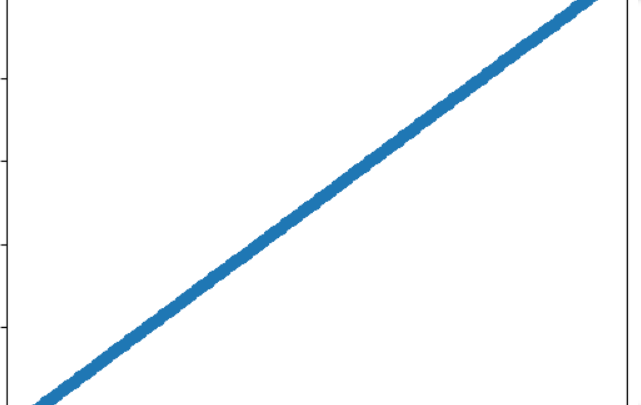
\includegraphics[width=0.5\linewidth]{image09.png}
    \caption{Random Scatter implementation}
    \label{fig:enter-label}
\end{figure}
\begin{figure}
    \centering
    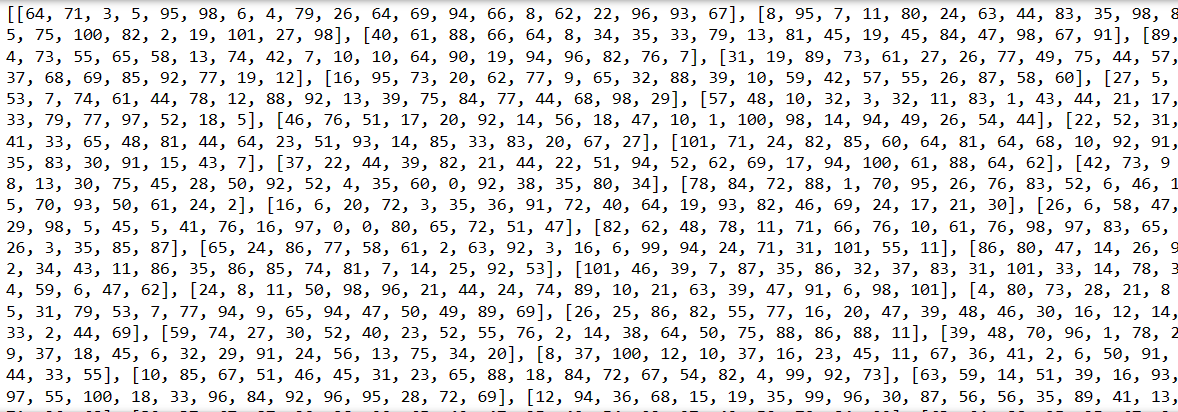
\includegraphics[width=0.5\linewidth]{please.png}
    \caption{Generated x and y values}
    \label{fig:enter-label}
\end{figure}

To implement gradient descent, the gradients for both the slope, "m", and intercept, "b", are declared as 0. A for loop will go through both arrays to pull the x and y value for each iteration. Using those values the gradient will be calculated using the formula found in the python code for both m and b. After the for loop is completed a new m and b will be returned. A loss function is used to know when the gradient descent no longer needs to be calculated. When the function is called it will return the mean squared of the loss found. 
\begin{figure}
    \centering
    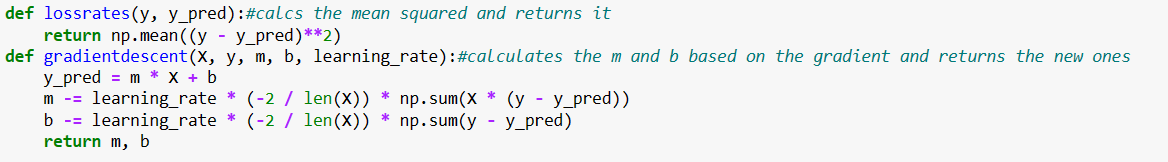
\includegraphics[width=0.5\linewidth]{asdasdasdwqa.png}
    \caption{Functions used for linear regression}
    \label{fig:enter-label}
\end{figure}
The while loop is what will take both functions and execute on the operations needed. The starting slope and intercept can be any value but for time sake it is preferred to keep it a reasonable number give that the generated x values are between one and one hundred. Based on the given threshold inputted by the user, the inner loop conditional will check to see if the threshold has been reached before breaking. This is because, at some point the reduction will be so minimal that there is no need to continue gradient descent.
\begin{figure}
    \centering
    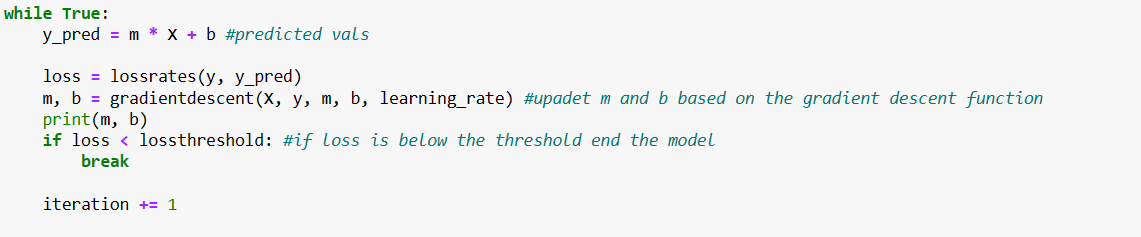
\includegraphics[width=0.5\linewidth]{asfwgsdgewrenrherher.png}
    \caption{While loop that will call on the function}
    \label{fig:enter-label}
\end{figure}
\begin{figure}
    \centering
    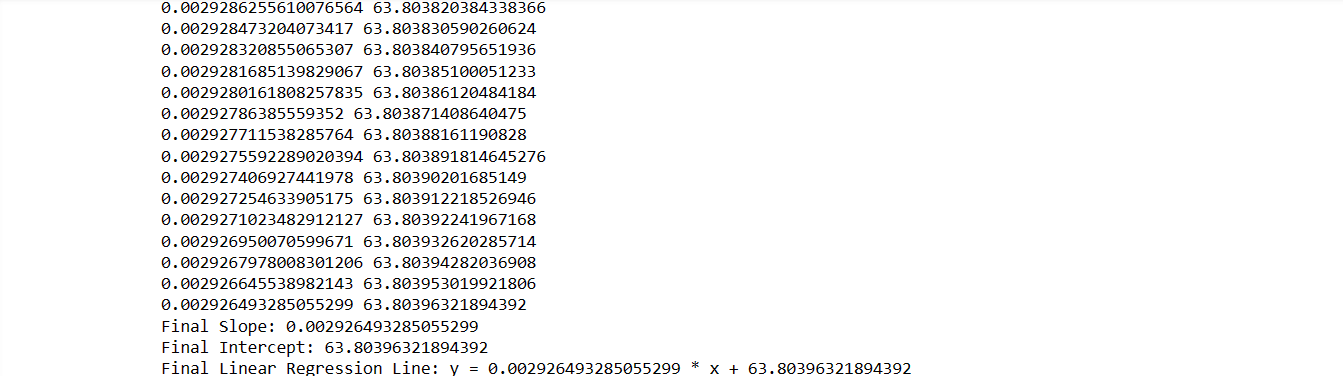
\includegraphics[width=0.5\linewidth]{aasdirututhgg.png}
    \caption{Final outputted text display}
    \label{fig:enter-label}
\end{figure}
Figure six displays the outputted changes for the slope and intercept with each iteration.
\begin{figure}
    \centering
    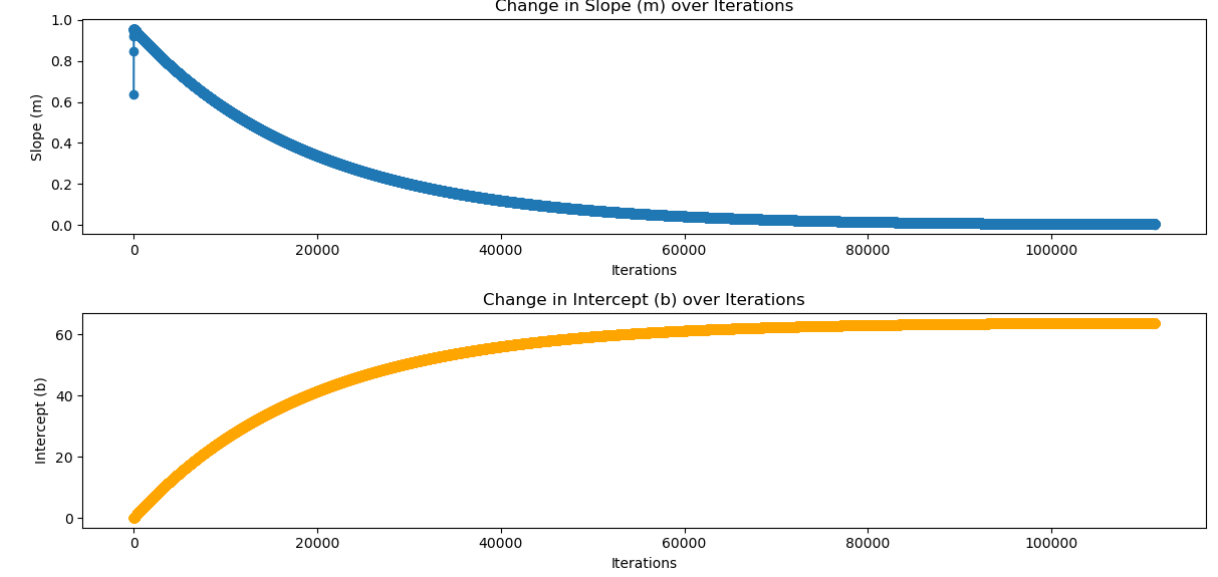
\includegraphics[width=0.5\linewidth]{changeplot.png}
    \caption{Changes for slop and intercept}
    \label{fig:enter-label}
\end{figure}
\section{Weka}
As stated previously, the produced csv file will be put into weka for comparison. Using the linear regression classifier gives the output in figure 7 and 8. From the scatter plot in the notebook to the visualization in figure 8, there is a striking similarity. Taking a look at the data summary, the correlation shows to be high, which can be expected based on looking at the scatter plot.
\begin{figure}
    \centering
    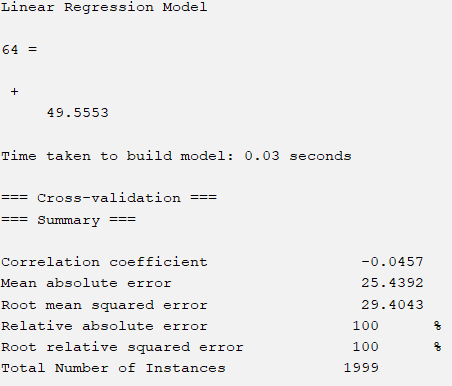
\includegraphics[width=0.5\linewidth]{yuikmnbvfdertyuj.png}
    \caption{Weka data output}
    \label{fig:enter-label}
\end{figure}
\begin{figure}
    \centering
    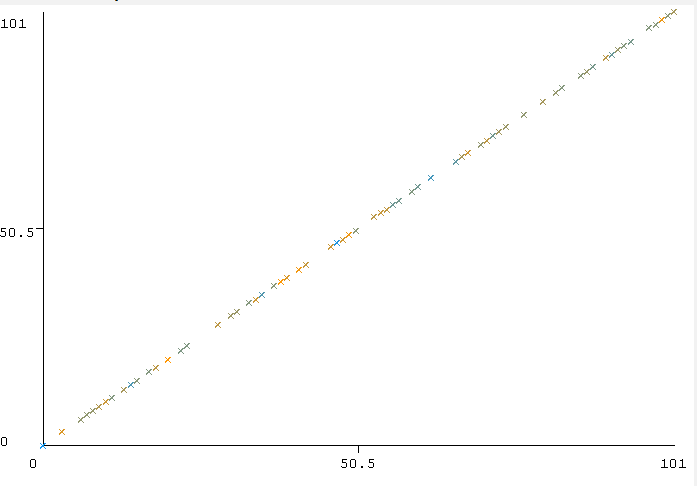
\includegraphics[width=0.5\linewidth]{image12.png}
    \caption{Visualization of data from csv of linear regression}
    \label{fig:enter-label}
\end{figure}
\section{Conclusion}
The purpose of the assignment was to implement linear regression from scratch to better understand how the model works. While the python implementation provided what was asked for, weka's provided information shows that this model is the best type for the given data set. This is because of the high correlation stemming from the random generation of x values. However, in some cases linear regression may not be the best model for the data set. It is important to understand the data and study it to use the best model for it.
\end{document}
